%%%%%%%%%%%%%%%%%%%%%%%%%%%%%%%%%%%%%%%%%%%%%%%%%%%%%%%%%%%%
\newcommand{\coursename}{Математический анализ 1 к. 2 с.}
\newcommand{\compiledby}{} % укажите свое имя
\newcommand{\coursedate}{Весна 2018 г.}
%%%%%%%%%%%%%%%%%%%%%%%%%%%%%%%%%%%%%%%%%%%%%%%%%%%%%%%%%%%%%%%%%%%%%%%%%%%%%%%%
% Преамбула для набора конспектов
% Версия 1.1
% Алексей Трошин. mailto: ai-troshin@yandex.ru

\documentclass[a4paper]{article}           % тип документа

\usepackage{geometry}     
              % задание полей текста
\geometry{left=30mm,right=10mm,top=20mm,bottom=20mm}
\usepackage[usenames]{color}
\usepackage{colortbl}
\usepackage{tikz}  
\usepackage{amsmath,amsfonts,amssymb}      % расширенная математика
\usepackage{xifthen}                       % удобный формат условий
\usepackage{graphicx}                      % поддержка рисунков
\usepackage{wrapfig}                       % поддержка обтекаемых рисунков
\usepackage{subcaption}                    % поддержка 'субрисунков'
\usepackage[makeroom]{cancel}              % поддержка зачеркиваний (сокращений)
\usepackage{ wasysym }
\usepackage{caption}                       % переопределение формата подписей
\captionsetup[figure]{labelsep=period}     % 'Рис. 1. ' вместо 'Рис. 1: '

\usepackage{unicode-math}                  % поддержка шрифта STIX Two
\defaultfontfeatures{Ligatures=TeX,Mapping=tex-text}
\setmainfont{STIX Two Text}
\setmathfont{STIX Two Math}

\usepackage{polyglossia}                   % поддержка языков в XeTeX
\setdefaultlanguage[spelling=modern]{russian}
\setotherlanguage{english}
\PolyglossiaSetup{russian}{indentfirst=true}

\sloppy                                    % строго соблюдать границы текста
\linespread{1.3}                           % коэффициент межстрочного интервала
\setlength{\parskip}{0.5em}                % вертик. интервал между абзацами

\setcounter{secnumdepth}{0}                % отключение нумерации разделов
\binoppenalty=1000                         % уменьшение переносов в формулах

\newcommand{\Def}{\textbf{Def.} }          % объявление новых макрокоманд

\newcommand{\Th}[1]{\textbf{Th\ifthenelse{\isempty{#1}}{}{ (#1)}.}}
\newcommand{\Consequence}[1]
           {\textbf{Следствие\ifthenelse{\isempty{#1}}{}{ #1}.}}
\newcommand{\Problem}[1]{\textbf{Задача\ifthenelse{\isempty{#1}}{}{ (#1)}.}}

\newcommand{\Remind}{\textbf{Напоминание.} }
\newcommand{\Note}{\textbf{Замечание.} }
\newcommand{\Statement}{\textbf{Утверждение.} }
\newcommand{\Proof}{\textbf{Доказательство:} }
\newcommand{\Prooff}{\textbf{Доказать:} }
\newcommand{\Solution}{\textbf{Решение.} }
\newcommand{\Endproof}{$\blacksquare$ }
\newcommand{\Endproofmath}{\ \blacksquare}
\newcommand{\Lemma}{\textbf{Лемма.} }
\newcommand{\Example}{\textbf{Пример:} }
\newcommand{\Examples}{\textbf{Примеры.} }


\newcommand{\ds}{\displaystyle}
\newcommand{\opn}{\operatorname}

\newcommand{\va}{\mathbfit{a}}             % макрокоманды для векторов: a,b,c,n
\newcommand{\vb}{\mathbfit{b}}
\newcommand{\vc}{\mathbfit{c}}
\newcommand{\vn}{\mathbfit{n}}

\newcommand{\holds}{\hookrightarrow}       % символ 'выполняется'
\newcommand{\N}{\mathbb{N}}                % символ множества N
\newcommand{\Z}{\mathbb{Z}}                % символ множества Z
\newcommand{\Q}{\mathbb{Q}}                % символ множества Q
\newcommand{\R}{\mathbb{R}}                % символ множества R
\newcommand{\U}{\text{U}}                  % символ окрестности
\newcommand{\Uo}{\text{Ů}}                 % символ проколотой окрестности
\newcommand{\lito}{\bar{\bar \textrm{o}}}  % символ 'o малое'
\newcommand{\bigo}{\textrm{O}}             % символ 'o большое'
\newcommand{\Ue}{\U_{\varepsilon}}
\newcommand{\Uoe}{\Uo_{\varepsilon}}

\newcommand{\eqdef}{\stackrel {\mathrm{def}}{=}}

\newcommand{\notimplies}{\ \nRightarrow\ } % символ 'не следует'

\newcommand{\eq}{\,=\,}
\newcommand{\todo}{\textbf {ВСТАВИТЬ ПРИМЕРЫ С РИСУНКАМИ!!!} }

\newcommand{\RNumb}[1]{\uppercase\expandafter{\romannumeral #1\relax}}

\renewcommand{\thefootnote}                % добавление ')' к номеру сноски
             {\arabic{footnote})}



\usepackage{titleps}                       % колонтитулы

\newpagestyle{main}{
  \setheadrule{.4pt}                       % линия отбивки верхнего колонтитула
  \sethead{\coursename}{}{\ifnum\thepage=1 % ЛУ, Ц, ПУ верхнего колонтитула
    \compiledby\else\sectiontitle\fi}
  \setfootrule{.4pt}                       % линия отбивки нижнего колонтитула
  \setfoot{\coursedate}{}{\thepage} }      % ЛУ, Ц, ПУ нижнего колонтитула

\pagestyle{main}

\newcommand{\Le}{\leqslant}                % русский стиль нестрогих неравенств
\newcommand{\Ge}{\geqslant}
%%%%%%%%%%%%%%%%%%%%%%%%%%%%%%%%%%%%%%%%%%%%%%%%%%%%%%%%%%%%%%%%%%%%%%%%%%%%%%%%

%%%%%%%%%%%%%%%%%%%%%%%%%%%%%%%%%%%%%%%%%%%%%%%%%%%%%%%%%%%%
\begin{document}

\section{Семинар №4}

\subsection{Рассматриваем функции в $\R^2$.}

\Def (предел $f(x,y)$ в точке $(x_0, y_0)$ по направлению $\vec l \,$).

~~\parbox[t]{0.95\linewidth} {
Пусть $f(x)$ определена в некоторой $\Uo(x_0, y_0)$ и пусть $\vec l (\cos\varphi, \sin\varphi)$ --- некоторый единичный вектор.
$$\lim\limits_{\substack {x \to x_0 \\ y \to y_0 \\ \normalsize \text{$(x,y)  \in  l(\varphi)$}}} \! \! \! \! \! \! \eqdef \lim\limits_{\rho \to +0} f(x_0 + \rho\cos\varphi,\, y_0 + \rho\sin\varphi) $$
}

\Note $l(\varphi) = \left\{ (x,y) \, | \, x=x_0 + \rho\cos\varphi,\, y=y_0 + \rho\sin\varphi, \, \rho \in (0, +\infty) \right\}$ --- луч.

\begin{figure}[h]
	\begin{center}
	    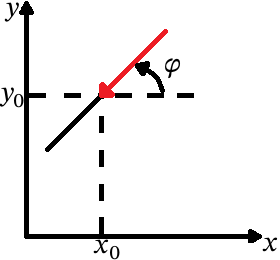
\includegraphics[width=0.25\textwidth]{1.png}
	  \end{center}
	\caption{}
\end{figure}

\Th {\textcolor{red}{\underline {\textcolor{black}{необходимое}}} условие $\boldsymbol {\exists \lim\limits_{\substack {x \to x_0 \\ y \to y_0}} f(x,y)}$}

~~$\exists \lim\limits_{\substack {x \to x_0 \\ y \to y_0}} f(x,y) = a \Rightarrow \forall \varphi \in [0, 2\pi) \; \exists \! \! \! \! \! \! \! \! \lim\limits_{\substack {x \to x_0 \\ y \to y_0 \\ \normalsize \text{$(x,y)  \in  l(\varphi)$}}} \! \! \! \! \! \! f(x,y) = a$

\Consequence{} $\lim\limits_{\substack {x \to x_0 \\ y \to y_0 \\ \normalsize \text{$(x,y)  \in  l(\varphi)$}}} \! \! \! \! \! \! f(x,y)$ зависит от $\varphi$ или $\nexists \Rightarrow \nexists \lim\limits_{\substack {x \to x_0 \\ y \to y_0}} f(x,y)$.

\Example $f(x,y) = \frac{xy}{x^2 + y^2}$. Исследовать $\exists$ - е $\lim\limits_{\substack {x \to x_0 \\ y \to y_0}} f(x,y) $.

~~Рассмотрим $\! \! \! \! \! \!  \lim\limits_{\substack {x \to x_0 \\ y \to y_0 \\ \normalsize \text{$(x,y)  \in  l(\varphi)$}}} \! \! \! \! \! \! f(x,y) = \lim\limits_{\rho \to +0} \frac {\cancel{\rho}\cos\varphi \cancel{\rho}\sin\varphi}{\cancel{\rho^2}\underbrace{(\cos^2\varphi + \sin^2\varphi)}_{1}} = \lim\limits_{\rho \to \infty} (\cos\varphi\sin\varphi) = \underbrace{\cos\varphi\sin\varphi}_{\text{зависит от } \varphi} \Rightarrow \nexists  \lim\limits_{\substack {x \to x_0 \\ y \to y_0}} f(x,y)$.

\Consequence{} $\forall \varphi \in [0, 2\pi) \exists \! \! \! \! \! \!  \lim\limits_{\substack {x \to x_0 \\ y \to y_0 \\ \normalsize \text{$(x,y)  \in  l(\varphi)$}}} \! \! \! \! \! \! f(x,y) = a  \cansel{\Rightarrow} \exists \lim\limits_{\substack {x \to x_0 \\ y \to y_0}} f(x,y) = a$. 





\end{document}